% https://arxiv.org/abs/2302.04742
\documentclass[a4paper,twocolumn,10pt]{article}

\usepackage{nopageno} % http://kb.mit.edu/confluence/pages/viewpage.action?pageId=3907018

\usepackage[english]{babel}
\usepackage[utf8]{inputenc} 
\usepackage{times} % Times font

\usepackage{cite} % https://www.overleaf.com/learn/latex/Bibliography_management_with_bibtex
\usepackage{url} % https://en.wikibooks.org/wiki/LaTeX/Hyperlinks#\url
\usepackage{anyfontsize} % https://texblog.org/2012/08/29/changing-the-font-size-in-latex/

\usepackage{mathtools} % https://en.wikibooks.org/wiki/LaTeX/Mathematics
\usepackage{amsmath}
\usepackage{amssymb} % https://www.cmor-faculty.rice.edu/~heinken/latex/symbols.pdf
\usepackage{siunitx} % https://tex.stackexchange.com/questions/59032/how-to-format-si-units

\usepackage[ruled,vlined,linesnumbered, noend, noline]{algorithm2e} % https://en.wikibooks.org/wiki/LaTeX/Algorithms
% https://mirror.szerverem.hu/ctan/macros/latex/contrib/algorithm2e/doc/algorithm2e.pdf

\usepackage{enumerate} % Meth or math
\usepackage{graphicx} % Insert images
\usepackage{geometry} 
\geometry{left=19mm, top=15mm, right=19mm, bottom=20mm} % Set the margins

\title{\textbf{A Vision-Based Algorithm for a Path Following Problem}}
\author{Mario Terlizzi$^{1}$, Giuseppe Silano$^{2}$, Luigi Russo$^{1}$, Muhammad Aatif$^{1}$,\\
Amin Basiri$^{1}$, Valerio Mariani$^{1}$, Luigi Iannelli$^{1}$, and Luigi Glielmo$^{1}$
    % https://tex.stackexchange.com/questions/4170/multiple-thanks-that-refer-to-same-text/4171#4171
    \thanks{This project was partially funded by the ECSEL Joint Undertaking (JU) research and innovation programme AFarCloud and COMP4DRONES under grant agreement no. 783221 and no. 826610, respectively, and by the European Union's Horizon 2020 research and innovation programme AERIAL-CORE under grant agreement no. 871479. The JU receives support from the European Union's Horizon 2020 research and innovation programme and Spain, Germany, Austria, Portugal, Sweden, Finland, Czech Republic, Poland, Italy, Latvia, Greece, and Norway.}
    \thanks{$^{1}$Mario Terlizzi, Luigi Russo, Muhammad Aatif, Amin Basiri, Valerio Mariani, Luigi Iannelli, and Luigi Glielmo are with the Department of Engineering, University of Sannio in Benevento, Benevento, Italy (email:  {\tt\small \{mterlizzi, luirusso, maatif, basiri, vmariani, luiannel, glielmo\}@unisannio.it}).}
    \thanks{$^{2}$Giuseppe Silano is with the Faculty of Electrical Engineering, Czech Technical University in Prague, Czech Republic (email: {\tt\small giuseppe.silano@fel.cvut.cz})}
}
\date{}

\begin{document}
\maketitle

    {\fontsize{9}{12}
    \textbf{\textit{Abstract} — A novel prize-winner algorithm designed for a path following problem within the Unmanned Aerial Vehicle (UAV) field is presented in this paper. The proposed approach exploits the advantages offered by the pure pursuing algorithm to set up an intuitive and simple control framework. A path for a quad-rotor UAV is obtained by using downward facing camera images implementing an Image-Based Visual Servoing (IBVS) approach. Numerical simulations in MATLAB{\textregistered} together with the MathWorks{\texttrademark} Virtual Reality (VR) toolbox demonstrate the validity and the effectiveness of the proposed solution. The code is released as open-source making it possible to go through any part of the system and to replicate the obtained results.\\
    \textit{Index Terms} — Path following, UAV, multi-rotor, virtual reality, image processing.}}

    \section{Introduction}
    % \label{sec:introduct}

    Path following is a relevant application problem within the Unmanned Aerial Vehicle (UAV) field. For instance, in precision agriculture scenarios having good path following algorithms is a fundamental requirement 
    to preserve high productivity rates and plant growth~\cite{1_basso2019uav}. In civilian applications, monitoring of power lines can be encoded as a path following problem between several target regions that need to be inspected~\cite{Silano2021ICRARAL}. Whatever the field of application is, drones have to follow a path to accomplish the mission specifications safely and successfully. 

    Looking at the path following problem, it can be divided into two parts: 
    \textit{detection} and \textit{path following}~\cite{Dahroug2018MARSS, Rafique2020TAES}. 
    As regards the \textit{path detection}, Hough transform~\cite{5_duda1972use} and its further 
    developments~\cite{6_duan2010improved, Du2010TIMP} are considered the most valuable solutions in the literature to cope with the task. However, such a transformation demands a high computational effort making it hard to run on-board the aircraft when battery and processing constraints are tight. These requirements are increasingly stringent when considering  Micro Aerial Vehicles (MAVs), where the sensor equipment and the vehicle dimensions are minimal. On the other hand, when the computational burden is at minimum, e.g., lightweight machine learning solutions have been recently proposed to tackle 
    the problem~\cite{7_van2019ls, Tang2021PR}, the time required to set up the algorithms makes them difficult to apply in real world applications. For all such reasons, it is of interest to have low computational intensity algorithms, possibly without any prior knowledge of the surrounding environment, able to provide references to the \textit{path following} in a given time window.

    \begin{figure}
        \centering
        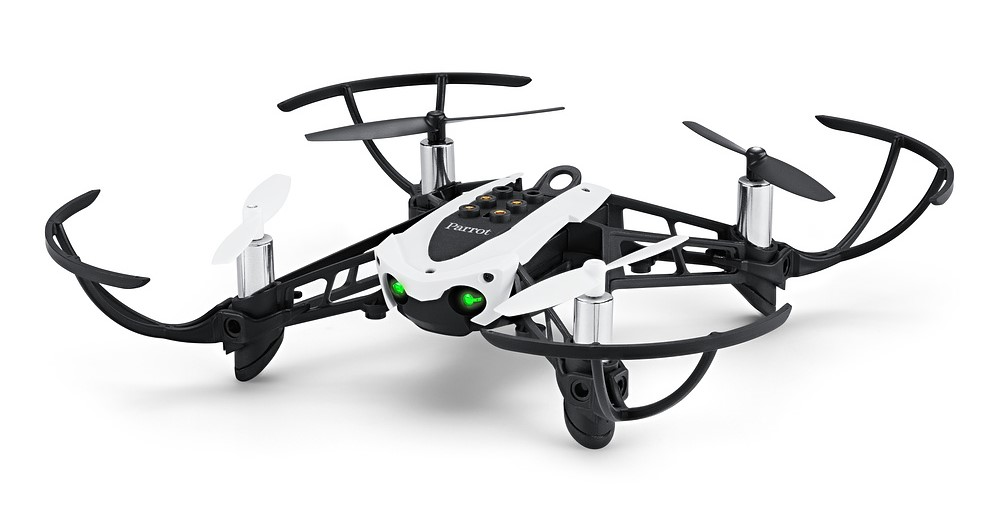
\includegraphics[width=0.3\textwidth]{pics/fig1_drone.jpg}
        \caption{Parrot Mambo quad-rotor~\cite{15_Mathworks_url}.}
        \label{fig:fig1Drone}
    \end{figure}

    Moving at the \textit{path following} level, much of the state-of-the-art 
    solutions~\cite{8_sujit2013evaluation, 12_pelizer2017comparison} rely on the use of nonlinear guidance law~\cite{Keshmiri2018ICUAS}, vector field~\cite{Tuttle2021ARC}, and pure 
    pursuit~\cite{Baqir2020IOP} algorithms due to their simple implementation and ease of use. Although the choice of path planner is application sensitive, general considerations can be provided. The performance of nonlinear guidance law degrades as the target acceleration changes rapidly introducing a not negligible delay in the trajectory generation. An adequate knowledge of the 
    target velocity and acceleration is required to avoid instability issues~\cite{Keshmiri2018ICUAS}. On the other hand, a vector field solution prevents from such oscillations problems, but it is 
    inherently characterized by a high computational effort~\cite{Tuttle2021ARC}. Besides, a pure pursuit approach is a suitable solution when tracking error and computational effort are critical. The position of a look-ahead point is set up at the beginning of the mission, and then updated at 
    each step following some tracking criteria~\cite{Gautam2015ICUAS, 10_xavier2019path, Silano2019SMC}. The objective is to reduce the distance between the current position and the look-ahead position.

    In this paper, we propose a novel winner-prize algorithm designed to deal with the path following problem in the context of the IFAC2020 MathWorks Minidrone 
    competition~\cite{4_Mathworks_url}. The framework combines the advantages provided by the pure pursuit algorithm and some simple image processing to detect and to track a pre-established path. The lightweight and ease of implementation of the proposed solution allow the deployment on low computational 
    capacity MAVs, such as the Parrot Mambo~\cite{15_Mathworks_url} (see, Figure~\ref{fig:fig1Drone}) considered as a testbed for the application. Numerical simulations 
    carried out in MATLAB together with the MathWorks Virtual Reality (VR) toolbox~\cite{SilanoMATFly} show the validity and the effectiveness of the proposed approach. Moreover, the code is provided as 
    open-source~\cite{GitHubCode} making it possible to go through any part of system and to replicate the obtained results. 

    The paper is organized as follows. Section~\ref{sec:probDesc} presents the problem, while in Sec.~\ref{sec:VisBasedFollow} the vision-based path following algorithm is 
    described. Numerical simulations are reported in Sec.~\ref{sec:NumRes}. Finally, conclusions are drawn in Sec.~\ref{sec:conclu}. 

    \section{Problem Description}
    \label{sec:probDesc}

    The work presented here finds an application within the IFAC2020 MathWorks Minidrone competition~\cite{4_Mathworks_url}, where the use of a model-based design approach is the aim of the specific contest. Path error and mission time are used as evaluation metrics for the algorithm. The whole process is the following: a quad-rotor UAV follows a pre-established red path by using its downward facing camera to get feedback from the environment. Images are updated according to the position and orientation of the vehicle simulated in the MATLAB VR world. No prior knowledge on the path and the surrounding scenario is given. The drone takes off and starts its  motion looking at the path, and the mission stops with the recognition of an end-marker. At that time, the drone lands staying within the delimited area. 
    Figure~\ref{fig:fig2track} shows the considered scenario. 

    \begin{figure}
        \centering
        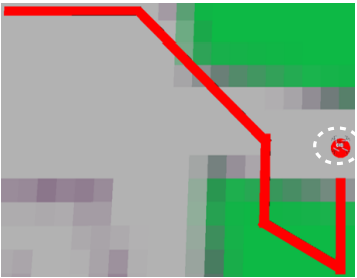
\includegraphics[width=0.3\textwidth]{pics/fig2_track.png}
        \caption{Snapshot extracted from the virtual scenario. A dashed circle is used to indicated the drone position.}
        \label{fig:fig2track}
    \end{figure}

    \section{Vision-Based Path Following Algorithm}
    \label{sec:VisBasedFollow}

    The vision-based path following algorithm combines the advantages offered by the pure pursuit algorithm~\cite{14_coulter1992implementation} with that of an easy image processing system to cope with the task. The algorithm starts selecting a target position ahead of the vehicle and that has to be reached, typically on a path. The framework is based on the following operations: (i) given 
    the actual position $\mathbf{d}=(x_d, y_d)^\top \in \mathbb{R}^2$ where the UAV is located, 
    a Virtual Target Point (VTP)  is set over the track at $\mathbf{w}=(x_w, y_w)^\top \in \mathbb{R}^2$; then, (ii) the quad-rotor is commanded to reach the VTP along a straight line (essentially it is the pure 
    pursuit algorithm with a curvature of infinite radius)~\cite{14_coulter1992implementation}, i.e., 
    moving the vehicle from its current position to the goal position\footnote{The quad-rotor is assumed to fly at a fixed height along the entire mission.}. 
    In Figure~\ref{fig:fig3path} an illustrative example of how the algorithm works is depicted. 

    \begin{figure}
        \centering
        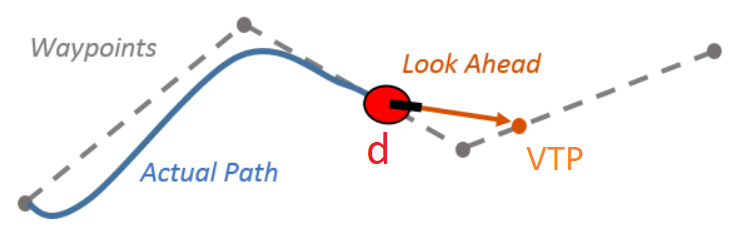
\includegraphics[width=0.49\textwidth]{pics/fig3_path.png}
        \caption{An illustrative example of the proposed vision-based path following algorithm works. 
        The red point $\mathbf{d}$ represents the drone position, while the orange point $\mathbf{w}$ 
        depicts the VTP.}
        \label{fig:fig3path}
    \end{figure}
    \begin{figure}
        \centering
        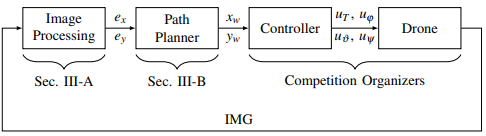
\includegraphics[width=0.49\textwidth]{pics/fig4_frick.png}
        \caption{Control system architecture. From left to right: the image processing, path planner, 
        controller, and drone blocks.}
        \label{fig:fig4diagram}
    \end{figure}

    Contrary to the pure pursuit algorithm, the proposed approach exploits the intrinsic 
    characteristics of the multi-rotor UAV motion: differently from ground vehicles with steering 
    wheels, drones can follow a path without modifying their heading. Such an assumption allows 
    reducing the time to accomplish the task by removing the control of the heading from the purposes 
    of the path follower.

    In Figure~\ref{fig:fig4diagram} the whole control scheme architecture is reported. The algorithm is mainly divided into two parts: (i) the Image Processing System (IPS) deals with extracting the red path from the 
    camera images, providing the errors along the $x$- and $y$-axis of the camera frame between the current drone position and the VTP point, and recognizing the End-Marker for the landing operations; while, (ii) the Path Planner (PP) figures out the path following problem by computing the new 
    position $\mathbf{w}$ of the drone in the world frame\cite[Sec.~V]{SilanoMATFly} implementing 
    an Image-Based Visual Servoing (IBVS) scheme. The control algorithm computes the commands $u_T$, $u_\varphi$, $u_\vartheta$, and $u_\psi$ that should be given to the drone in order to update its position and orientation in accordance to the PP references. 

    The overall mission is divided into four parts: \textit{Take off}, \textit{Following}, \textit{End-Marker}, and \textit{Landing}. A decision-making process has been implemented to  achieve the competition objectives triggering the system from a state to another, as depicted in 
    Figure~\ref{fig:fig5stateMachine}. For each frame, the IPS accesses the system status and plan the next action (i.e., landing, following, etc.). The drone starts taking off from its initial position looking at the path. Once the vehicle reaches the hovering position, the IPS detects the path and the state machine enters in the \textit{Following} state, hence the path following starts. As soon as the IPS detects the End-Marker, the state machine exits from the \textit{Following} state and goes into the \textit{End-Marker} state. At this stage the mission stops, and the drone starts the landing. In the following subsections the implementation of the image processing system and path planner modules are detailed.

    \pagebreak
    \subsection{Image processing system}
    % \label{sec:imageProcSys}

    \begin{figure}
        \centering
        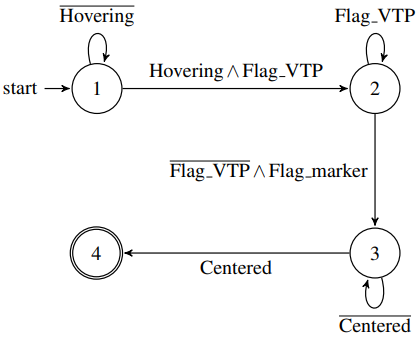
\includegraphics[width=0.49\textwidth]{pics/fig5_lines.png}
        \caption{State machine implemented. State 1: \textit{Take-off}. State 2: \textit{Following}. State 3: \textit{End-Marker}. State 4: \textit{Landing}.} 
        \label{fig:fig5stateMachine}
    \end{figure} 

    Starting from the camera frames, the Image Processing System takes care of separating the features of the 
    pre-established path from that of the environment.
    The IPS receives frames of width $W$ and height $H$ from the camera sensor at each   
    $T_\mathrm{IPS} = 0.2$s, i.e., the camera sampling time. The image format is RGB with 
    $8$ bits for each color channel. The path is 0.01 m in width, while the landing marker 
    is circular with a diameter of 0.02 m. The path color is red, and this information is 
    taken into consideration in all the elaborations to filter out the background scenario. The 
    procedure consists of the following steps: first, the RGB frame is converted into an intensity 
    level frame representation as follows 
    \begin{equation}
        F(n,m)=f_R(n,m) -  \frac{f_G(n,m)}{GG} - \frac{f_B(n,m)}{GB} ,
    \end{equation}
    where the pair $(n,m)$ represents the pixel located at row $n \in \{1, 2, \dots, H\}$ and column $m 
    \in \{1, 2, \dots, W\}$ of the image frame and $f_i$, with $i \in \{R, G, B\}$, provides the intensity level representation of the corresponding red, green and blue channels. An heuristic 
    approach was used to tune the $GG$, $GB \geq 1$ parameter values. These parameters help to detect the pixels belonging to the path. Further, a binarization process based on a $K_T$  threshold value refines the process removing artifacts from the elaboration. The binarized frame can be described by the binary 
    function $F_\mathrm{bin} \colon (n,m) \to \{0, 1\}$ whose output is one when the pixel belongs to the path and zero otherwise. Finally, an erosion operation is performed through a 
    square kernel to shrink and regularize the binarized frame. In Figure~\ref{fig:fig6frames} the overall process is reported for a single sample frame.

    \begin{figure}
        \centering
        
\includegraphics[width=0.49\textwidth]{pics/fig6_track.jpg}
        \caption{Original frame (upper left),  converted and binarized frame (upper right), and eroded frame (lower).}
        \label{fig:fig6frames}
    \end{figure}

    Then, the obtained reference path is used in a twofold way: (i) to identify a new VTP belonging to the track; (ii) to detect the landing marker. The two tasks are described in the 
    pseudocode reported in Algorithm~\ref{alg:ImgProc}.

    Looking at the algorithm, the first three functions (i.e., \texttt{channelConv}, \texttt{binarization}, and \texttt{erosion}) take care of extracting the path information from the frame. Then, the \texttt{detectTrack} and \texttt{detectMarker} functions deal with raising a flag when the path (\texttt{Flag\_VTP}) or the End-Marker (\texttt{Flag\_marker}) are detected. The path following algorithm starts with the IPS that computes the errors ($e_x$ and $e_y$) between the drone position and the VTP point for the PP by using a circular arc mask centered in the 
    drone Center of Mass (CoM)\footnote{The assumption that the CoM being in the center of the reference 
    frame, i.e., $x_\mathrm{CoM} = \frac{H}{2}$ and $y_\mathrm{CoM}=\frac{W}{2}$, is taken into consideration.} with thickness $R_\mathrm{max} - R_\mathrm{min}$
    \footnote{$R_\mathrm{max}$ and $R_\mathrm{min}$ are the outer and inner radius, respectively.}. 

    In Figure~\ref{fig:fig7arcMask}, the arc mask considering the VTP position at time $\mathbf{t}_k$ 
    is depicted, where $\mathbf{t}_k$ denotes the $k$-element of the time interval vector defined as 
    $\mathbf{t} =(0, T_\mathrm{IPS}, \dots, NT_\mathrm{IPS})^\top \in \mathbb{R}^{N+1}$, with $k \in 
    \mathbb{N}_0$. The orientation angle \mbox{$\vartheta = \arctan$2$(x_\mathrm{VTP},y_\mathrm{VTP})$} 
    is calculated with respect to the frame coordinates, where the $\arctan$2 function is the 
    four-quadrant inverse of the tangent function. A portion~$\varTheta$ of the arc mask is established 
    by taking into account the previous VTP's orientation. In particular, we set up two semi-arcs 
    with width~$\frac{\varTheta}{2}$, namely Field of View (FoV), in counter-clockwise and clockwise 
    directions from $\vartheta$. Then, the arc mask is applied to the eroded image obtaining 
    the VTP point at $\mathbf{t}_{k+1}$. The function TP calculates $x_\mathrm{VTP}$, 
    $y_\mathrm{VTP}$, and $\vartheta$ which represent the frame coordinates and angle orientation of 
    the VTP at  $\mathbf{t}_{k+1}$, respectively. Subsequently the corresponding errors with 
    respect to the center of mass, i.e., $e_x$ and $e_y$, are computed inside the frame coordinates. 
    Finally, the \texttt{Flag\_VTP} and the $e_x$ and $e_y$ values are provided as input to the PP 
    at each $T_\mathrm{IPS}$. Figure~\ref{fig:fig8frames} shows the result of the entire process setup. 

    % https://en.wikibooks.org/wiki/LaTeX/Command_Glossary#Q
    \begin{algorithm}
        \caption{Image Processing System}
        \label{alg:ImgProc}
        $\text{IMG}  \gets \text{channelConv(\text{IMG})}$, \\
        $\text{IMG} \gets \text{binarization(\text{IMG})}$, \\
        $\text{IMG} \gets \text{erosion(\text{IMG})}$, \\
        $\text{Flag\_VTP} \gets \text{detectTrack(\text{IMG})}$, \\
        $\text{Flag\_marker}$ $\gets \text{detectMarker(\text{IMG})}$ \\
        \If {$\text{Flag\_VTP}$} {
            \quad $x_\mathrm{VTP} \text{, } y_\mathrm{VTP} \gets \text{vtp(frame)}$ \\
            \quad $e_x \gets x_\mathrm{VTP} - x_\mathrm{CoM}$ \\
            \quad $e_y \gets y_\mathrm{VTP} - y_\mathrm{CoM}$ \\
        }
        \Else{
            \If{$\text{Flag\_marker}$} {
            \qquad $\;$ $x_\mathrm{MARK}$, $y_\mathrm{MARK} \gets \text{cgMarker(frame)}$ \\
            \qquad $\;$ $e_x \gets x_\mathrm{MARK} - x_\mathrm{CoM}$ \\ 
            \qquad $\;$ $e_y \gets y_{\rm MARK} - y_{\rm CoM}$
            }
        }
        \Return $e_x$, $e_y$, $\text{Flag\_VTP}, \text{Flag\_marker}$ 
    \end{algorithm}
    The Path Planner is designed to compute the position of the VTP point $\mathbf{w} = (x_w, y_w)^\top$ maintaining a constant altitude ($z_H$) while following the path. Roughly speaking, the PP computes the spatial coordinates $x_w$ and $y_w$ trying to reduce the errors, i.e., $e_x$ and $e_y$, between the drone position and the VTP. These values are later used by the drone controller to tune the command signals $u_T$, $u_\varphi$, $u_\vartheta$, and $u_\psi$, as 
    described in Figure~\ref{fig:fig4diagram}. The proposed path planner is based on Proportial-Integra control loops. As a common rule in cascade structure, the inner loop, i.e., the PP, is regulated at a 
    rate faster than the outer loop, i.e., the IPS. In our case, the PP runs at 200 Hz ($T_\mathrm{PP} = 5X10^{-3}$s) while the IPS runs at 2 Hz ($T_\mathrm{IPS} = 0.2$s). These are a standard solution in the 
    literature for quad-rotors control design~\cite{Dief2015}.
    \begin{figure}
        \centering
        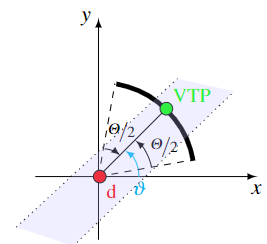
\includegraphics{pics/fig7_no.png}
        \caption{Arc mask. The drone position (red), the previous VTP (green), and the pre-established path to follow (purple) are reported.} 
        \label{fig:fig7arcMask}
    \end{figure}

    It is worth noticing that when the landing marker is detected and no other VTP point is found in the frame, the IPS triggers the state machine in the \texttt{End-Marker} state. Here, the new main task of the IPS is to obtain the position of the End-Marker within the frame coordinates. An additional erosion process is performed by using a circular kernel, as depicted in 
    Figure~\ref{fig:fig9frame}. 

    \subsection{Path planner}
    \label{sec:pathPlan}

    As described in Sec.~\ref{sec:VisBasedFollow}, the path following stops with the detection of the End-Marker. At that time, the IPS implements a toggle switch behavior raising the \texttt{Flag\_marker} flag while holding low the \texttt{Flag\_VTP} flag. This mutually separates the \textit{Following} and \textit{Landing} phases avoiding instability issues. The 
    pseudocode of the proposed algorithm is reported in Algorithm~\ref{alg:pathPlanAlg} with parameter 
    values detailed in Table~\ref{tab:paramTable}.

    \begin{figure}
        \centering
        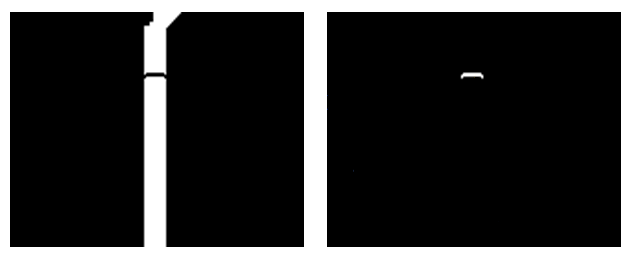
\includegraphics[width=0.49\textwidth]{pics/fig8_frame.png}
        \caption{Frame after the application of the Arc mask (left). Extracted pixels belonging to the 
        path (right).}
        \label{fig:fig8frames}
    \end{figure}
    \begin{figure}
        \centering
        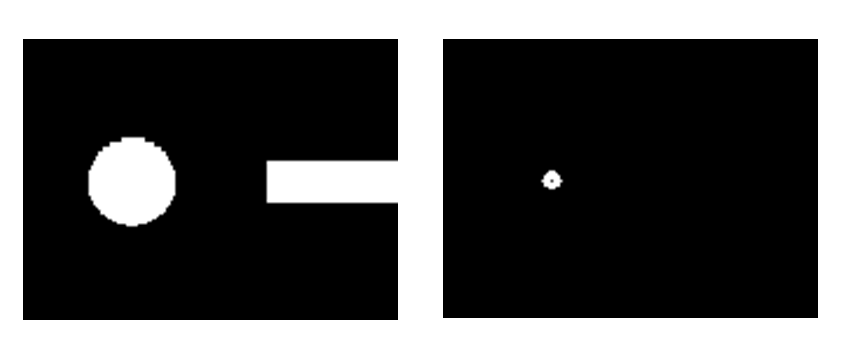
\includegraphics[width=0.49\textwidth]{pics/fig9_frame.png}
        \caption{Original (left) and eroded frames (right) of the End-Marker are reported.}
        \label{fig:fig9frame}
    \end{figure}

    In Appendix~\ref{append}, we show how $\alpha$ can be set to control the velocity of vehicle along the entire mission. Therefore, the proposed Vision-Based Path Following algorithm makes it possible not only to generate the spatial coordinates $x_w$ and $y_w$ using a IBVS scheme but also to set the velocity during the entire mission.

    \section{Numerical Results}
    \label{sec:NumRes}

    To demonstrate the validity and effectiveness of the proposed framework, numerical simulations have been carried out by using the 2019b release of MATLAB equipped with MathWorks Virtual Reality 
    toolbox~\cite{16_Mathworks_url} and Parrot support package for Simulink~\cite{15_Mathworks_url}. 
    The video available at~\cite{YouTubeVideo} illustrates in a direct way how the system works, i.e., the ability of the quad-rotor UAV to follow the pre-established red path and to land on the End-Marker. In addition, the video shows the behavior of the IPS and PP that never lose the path during the entire mission. 

    In Figure~\ref{fig:fig10graphs} a comparison of the system performance by using various values of $\alpha$ is reported. As can be seen from the plots, the larger $\alpha$ is, the lower the mission time ($T_s$) is. On the other hand, the lower the mission time is, the greater the path 
    error is. Looking at the zoom plot (see, Figure~\ref{fig:fig10graphs}) it is even clearer how the system performance degrades with increasing $\alpha$ value, and these are all the more evident as the path is angular. For the considered scenario, an heuristic approach was used to tune the $\alpha$ and $\beta$ parameter values.

    \begin{algorithm}
        \caption{Path Planner}
        \label{alg:pathPlanAlg}
        $e_x$, $e_y$, $\text{Flag\_VTP}$, $\text{Flag\_marker}$ \\
        \If{$\text{Flag\_VTP}$} {
            \quad $x_{k+1} \gets x_k + \alpha e_x$\\
            \quad $y_{k+1} \gets y_k + \alpha e_y$\\
            \quad $z_{k+1} \gets  z_H$
        }
        \If{$\text{Flag\_marker}$} {
            \If{$(e_x=0 \wedge e_y=0)$} {
            \qquad $\;$ $x_{k+1}  \gets x_k $\\
            \qquad $\;$ $y_{k+1} \gets y_k $\\
            \qquad $\;$ $z_{k+1} \gets 0$
            }
            \Else {
            \qquad $\;$ $x_{k+1} \gets x_k + \beta e_x$\\
            \qquad $\;$ $y_{k+1}  \gets y_k + \beta e_y$\\
            \qquad $\;$ $z_{k+1} \gets z_H$
            }
        }
        $x_w \gets x_{k+1}$, $y_w \gets y_{k+1}$, $z_w \gets z_{k+1}$ \\
        \Return $x_w$, $y_w$, $z_w$
    \end{algorithm} 
    \begin{table}
        \centering
        \caption{Parameter values.}
        \label{tab:paramTable}
        \footnotesize\begin{tabular}[t]{|l|l|c|c|}
            \hline
            & \textbf{Sym} & \textbf{Value}\\
            \hline
            Sampling time & $T_{\rm PP}$ & \num{5e-3} s\\
            Sampling time & $T_{\rm IPS}$ & 0.2s\\
            PP constant & $\beta$ & \num{18e-3} pixel$^{-1}$\\
            Frame height & $H$ & 120 pixel\\
            Frame width & $W$ & 160 pixel\\
            Outer radius Arc mask & $R_{\rm max}$ & 28 pixel \\
            Inner radius Arc mask & $R_{\rm min}$ & 26 pixel \\
            IPS constant & $GB$ & 2 \\
            IPS constant & $GG$ & 2 \\
            IPS threshold & $K_T$ & 150 \\
            FOV Arc mask & $\vartheta$ & 2.3 \si{\radian} \\
            Drone height & $z_H$ & 1 \si{\metre} \\
            \hline
        \end{tabular}
    \end{table}

    Figure~\ref{fig:fig11graph} depicts the drone velocity $v_x$ and $v_y$ along the $x$- and $y$-axis, respectively, and the norm of the drone velocity $v_D$. As described in 
    Sec.~\ref{sec:pathPlan} and detailed in Appendix~\ref{append}, the norm of the drone velocity remains approximately constant while following the path. The presence of spikes might be due to the coupling effects of the drone $xy$ dynamics even though $x_w$ and $y_w$ references have not been 
    modified yet (see, Figure~\ref{fig:fig10graphs}). Such coupling effects are probably caused by the asymmetric positioning of the rotors with respect to the principal axis and the effect of the discrete image pixelization. 

    \section{Conclusion}
    \label{sec:conclu}
    In this paper, a prize-winner algorithm designed for a path following problem within the IFAC2020 Mathworks Minidrone Competition has been presented. In particular, a lightweight and easy of implementation solution was set to generate the spatial coordinates of the VTP point to fulfill the competition requirements successfully. Numerical simulations carried out in MATLAB together with the MathWorks Virtual Reality toolbox and the Parrot support package for Simulink demonstrated the validity and the effectiveness of the proposed approach. The software has been released as open-source making it possible to go through any part of the system and to replicate the obtained results. Future work will include the integration of more challenging features, such as obstacle avoidance and 3-D reference generation, and lead to field experiments. Furthermore, the effects of the drone dynamics on the performance of the vision-based system will be also explored. 
    \begin{figure}
        \centering
        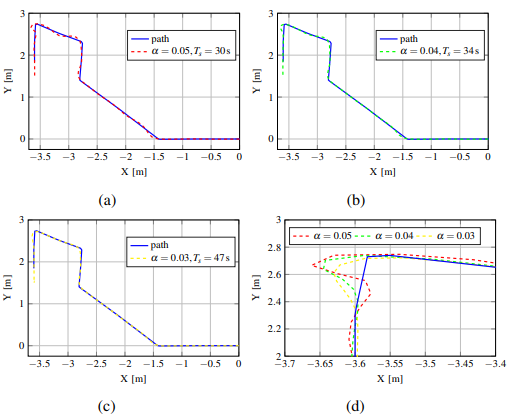
\includegraphics[width=0.49\textwidth]{pics/fig10_graph.png}
        \caption{Trajectory plots. From left to right: the desired and the drone paths for various values of $\alpha$ are represented. The mission time $T_s$ and a comparison between the considered $\alpha$ values are also reported.}
        \label{fig:fig10graphs}
    \end{figure}
    \begin{figure}
        \centering
        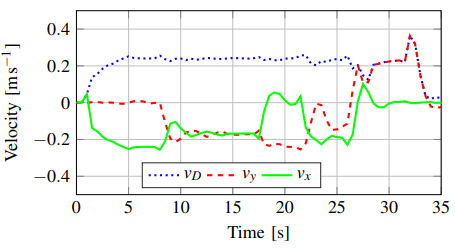
\includegraphics[width=0.49\textwidth]{pics/fig11_graph.png}
        \caption{Velocity plot.}
        \label{fig:fig11graph}
    \end{figure}

    \bibliographystyle{abbrv}
    \footnotesize\begin{thebibliography}{10}
        \bibitem{1_basso2019uav}
        B.~Maik and d.~E. Pignaton, ``{A UAV guidance system using crop row detection
        and line follower algorithms},'' \emph{Journal of Intelligent \& Robotic
        Systems}, pp. 1--17, 2019.

        \bibitem{Silano2021ICRARAL}
        G.~{Silano}, T.~{Baca}, R.~{Penicka}, D.~{Liuzza}, and M.~{Saska}, ``{Power
        Line Inspection Tasks with Multi-Aerial Robot Systems via Signal Temporal
        Logic Specifications},'' \emph{IEEE Robotics and Automation Letters}, vol.~6,
        no.~2, pp. 4169--4176, 2021.

        \bibitem{Dahroug2018MARSS}
        B.~Dahroug, J.-A. Séon, A.~Oulmas, T.~Xu, B.~Tamadazte, N.~Andreff, and
        S.~Régnier, ``{Some Examples of Path Following in Microrobotics},'' in
        \emph{International Conference on Manipulation, Automation and Robotics at
        Small Scales}, 2018, pp. 1--6.

        \bibitem{Rafique2020TAES}
        M.~A. Rafique and A.~F. Lynch, ``{Output-Feedback Image-Based Visual Servoing
        for Multirotor Unmanned Aerial Vehicle Line Following},'' \emph{IEEE
        Transactions on Aerospace and Electronic Systems}, vol.~56, no.~4, pp.
        3182--3196, 2020.

        \bibitem{5_duda1972use}
        R.~O. {Duda} and P.~E. {Hart}, ``{Use of the Hough transformation to detect
        lines and curves in pictures},'' \emph{{Communications of the ACM}}, vol.~15,
        no.~1, pp. 11--15, 1972.

        \bibitem{6_duan2010improved}
        D.~Dagao, X.~Meng, M.~Qian, H.~Zhongming, and W.~Yueliang, ``{An improved Hough
        transform for line detection},'' in \emph{2010 International Conference on
        Computer Application and System Modeling}, vol.~2, 2010, pp. V2--354.

        \bibitem{Du2010TIMP}
        S.~{Du}, B.~J. {van Wyk}, C.~{Tu}, and X.~{Zhang}, ``{An Improved Hough
        Transform Neighborhood Map for Straight Line Segments},'' \emph{IEEE
        Transactions on Image Processing}, vol.~19, no.~3, pp. 573--585, 2010.

        \bibitem{7_van2019ls}
        V.~Nhan, J.~Robert, and R.~Davide, ``{LS-Net: Fast Single-Shot Line-Segment
        Detector},'' \emph{Machine Vision and Applications}, vol.~12, no.~32, 2020.

        \bibitem{Tang2021PR}
        J.~{Tang}, S.~{Li}, and P.~{Liu}, ``{A review of lane detection methods based
        on deep learning},'' \emph{Patter Recognition}, vol. 111, pp. 1--15, 2021.

        \bibitem{8_sujit2013evaluation}
        P.~{Sujit}, S.~{Saripalli}, and J.~B. {Sousa}, ``{An evaluation of UAV path
        following algorithms},'' in \emph{2013 European Control Conference}, 2013,
        pp. 3332--3337.

        \bibitem{12_pelizer2017comparison}
        G.~V. {Pelizer}, N.~B. {Da Silva}, and K.~R. {Branco}, ``{Comparison of 3d
        path-following algorithms for unmanned aerial vehicles},'' in \emph{2017
        International Conference on Unmanned Aircraft Systems}, 2017, pp. 498--505.

        \bibitem{Keshmiri2018ICUAS}
        S.~{Keshmiri}, A.~R. {Kim}, D.~{Shukla}, A.~{Blevins}, and M.~{Ewing},
        ``{Flight Test Validation of Collision and Obstacle Avoidance in Fixed-Wing
        UASs with High Speeds Using Morphing Potential Field},'' in \emph{2018
        International Conference on Unmanned Aircraft Systems}, 2018, pp. 589--598.

        \bibitem{Tuttle2021ARC}
        T.~{Tuttle}, T.~T. {Moleski}, and J.~{Wilhelm}, ``{Multi-Rotor Path-following
        Performance using Vector Field Guidance and Velocity Control},'' in
        \emph{AIAA Scitech 2021 Forum}, 2021.

        \bibitem{Baqir2020IOP}
        A.~S. {Baqir} and A.~A. {Ammar}, ``{Navigation of Mini Unmanned Aerial Vehicle
        in Unknown Environment},'' \emph{IOP Conference Series: Materials Science and
        Engineering}, vol. 745, 2020.

        \bibitem{Gautam2015ICUAS}
        A.~{Gautam}, P.~B. {Sujit}, and S.~{Saripalli}, ``{Application of guidance laws
        to quadrotor landing},'' in \emph{2015 International Conference on Unmanned
        Aircraft Systems}, 2015, pp. 372--379.

        \bibitem{10_xavier2019path}
        D.~M. {Xavier}, B.~F.~S. {Natassya}, and R.~{Branco Kalinka}, ``{Path-following
        algorithms comparison using Software-in-the-Loop simulations for UAVs},'' in
        \emph{2019 IEEE Symposium on Computers and Communications}, 2019, pp.
        1216--1221.

        \bibitem{Silano2019SMC}
        G.~{Silano}, P.~{Oppido}, and L.~{Iannelli}, ``{Software-in-the-loop simulation
        for improving flight control system design: a quadrotor case study},'' in
        \emph{IEEE International Conference on Systems, Man and Cybernetics}, 2019,
        pp. 466--471.

        \bibitem{15_Mathworks_url}
        {MathWorks}, ``{Simulink Support Package for Parrot Minidrones}.'' [Online].
        Available:
        \url{https://www.mathworks.com/matlabcentral/fileexchange/63318-simulink-support-package-for-parrot-minidrones}

        \bibitem{4_Mathworks_url}
        Mathworks, \emph{{Mathworks Minidrone Competition IFAC20}}. [Online].
        Available:
        \url{https://it.mathworks.com/academia/student-competitions/minidrones/ifac-2020.html}

        \bibitem{SilanoMATFly}
        G.~Silano and L.~Iannelli, ``{MAT-Fly: An Educational Platform for Simulating
        Unmanned Aerial Vehicles Aimed to Detect and Track Moving Objects},''
        \emph{IEEE Access}, vol.~9, pp. 39\,333--39\,343, 2021.

        \bibitem{GitHubCode}
        M.~{Terlizzi}, ``{Vision Based Pure Pursuing Algorithm},'' GitHub repository.
        [Online]. Available:
        \url{https://github.com/mar4945/Vision-Based-Pure-Pursuing-Algorithm}

        \bibitem{14_coulter1992implementation}
        R.~C. {Coulter}, ``{Implementation of the pure pursuit path tracking
        algorithm},'' {Carnegie-Mellon UNIV Pittsburgh PA Robotics INST}, Tech. Rep.,
        1992. [Online]. Available:
        \url{http://www.enseignement.polytechnique.fr/profs/informatique/Eric.Goubault/MRIS/coulter_r_craig_1992_1.pdf}

        \bibitem{Dief2015}
        T.~N. Dief and S.~Yoshida, ``{Review: Modeling and Classical Controller Of
        Quad-rotor},'' \emph{International Journal of Computer Science and
        Information Technology \& Security}, vol.~5, no.~4, pp. 314--319, 2015.

        \bibitem{16_Mathworks_url}
        {MathWorks}, ``{Simulink 3D Animation toolbox}.'' [Online]. Available:
        \url{https://www.mathworks.com/products/3d-animation.html}

        \bibitem{YouTubeVideo}
        M.~{Terlizzi}, ``{MATLAB Minidrone Competition IFAC20},'' YouTube. [Online].
        Available: \url{https://youtu.be/9VySp0j-1hc}
    \end{thebibliography}

    \begin{appendix}
        \centering{\large{Appendix I}}
        \label{append}
        
        Let us consider a continuous-time dynamical system $\mathcal{H}$ and its discrete time version 
        $x_{k+1}=f(x_k,u_k)$, where $x_k, x_{k+1} \in X \subset \mathbb{R}^n$ are the current state and 
        the next state of the system, respectively, $u \in U \subset \mathbb{R}^m$ is the control 
        input. Let us consider the PP algorithm implementation detailed in 
        Algorithm~\ref{alg:pathPlanAlg}. Hence, the next state of the system $x_{k+1}$ and $y_{k+1}$ 
        along the $x$- and $y$-axis can be written as follows:
        \begin{equation}
            x_{k+1} = x_k + \alpha e_{x_k}, \qquad y_{k+1} = y_k + \alpha e_{y_k},
        \end{equation}
        respectively. After some simple algebra, we can write:
        \begin{equation}
            \dfrac{x_{k+1}-x_k}{T_{\rm PP}} = \dfrac{\alpha e_{x_k}}{T_{\rm PP}}, \qquad 
            \dfrac{y_{k+1}-y_k}{T_{\rm PP}} = \dfrac{\alpha e_{y_k}}{T_{\rm PP}}, 
        \end{equation}
        and hence,
        \begin{equation}
            v_x \approx \dfrac{\alpha e_{x_k}}{T_{\rm PP}} = \tilde{\alpha} e_{x_k}, \qquad 
            v_y  \approx  \dfrac{\alpha e_{y_k}}{T_{\rm PP}} = \tilde{\alpha} e_{y_k},
        \end{equation}
        with $\tilde{\alpha} = \frac{\alpha}{T_{\rm PP}}$.
        
        Knowing that $e_{x_k}$ and $e_{y_k}$ are by definition the projections over a circle along the 
        $x$- and $y$-axis of the VTP with an angle $\vartheta_k$, we can write
        \begin{equation}
            \begin{array}{rll}
                e_{x_k} &=& \dfrac{R_\mathrm{max}+R_\mathrm{min}}{2} \sin{\vartheta_k},\\[10pt]
                e_{y_k} &=& \dfrac{R_\mathrm{max}+R_\mathrm{min}}{2} \cos{\vartheta_k},
            \end{array}
        \end{equation}
        and thus,
        \begin{equation} 
            \begin{split}
                V_D & = \sqrt{v_x^2 + v_y^2} \approx \tilde{\alpha} 
                \dfrac{R_\mathrm{max}+R_\mathrm{min}}{2}. \\
            \end{split}
        \end{equation}
        Hence the parameter $\alpha$ controls the drone velocity. 
        \hspace*{\fill} $\blacksquare$ 
    \end{appendix}

\end{document}